\section{System}
\label{sec:sys}

\begin{figure}[t!]
\begin{center}
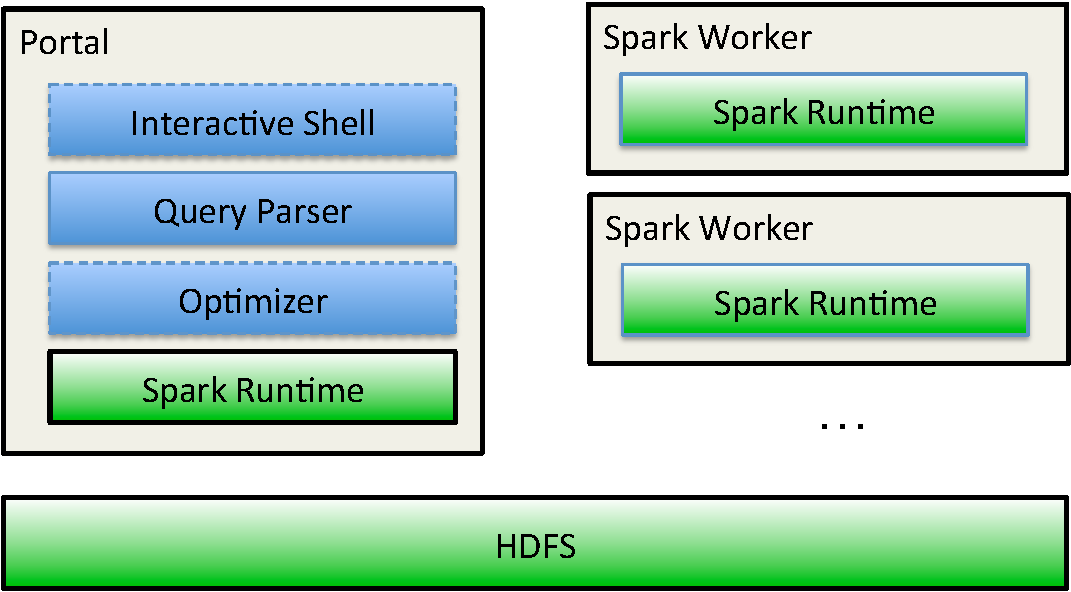
\includegraphics[height=1.4in]{figs/architecture.pdf}
\caption{\ql system architecture.}
\label{fig:arch}
\end{center}
\end{figure}

Our \ql system implementation builds on GraphX, an Apache Spark
library, as depicted in Figure~\ref{fig:arch}.  Green boxes indicate
built-in components, while blue are those we added for \ql.  We
selected Apache Spark because it is a popular open-source system, and
because of its in-memory processing approach.  All language operators
are available through the public API of the \ql library, and may be
used like any other library in an Apache Spark application.

\begin{figure}[t!]
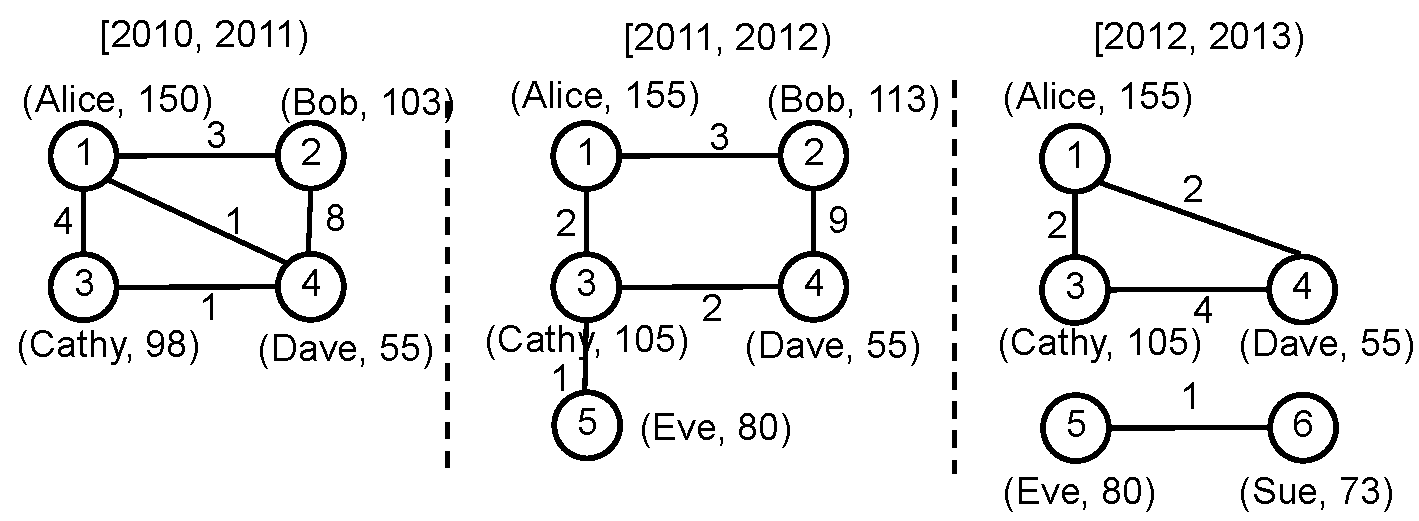
\includegraphics[width=3.2in]{figs/sgp.pdf}
\caption{SG representation of T1 from Figure~\ref{fig:tg}.}
\label{fig:sgp}
\end{figure}

The \ql system includes an interactive shell for exploratory data
analysis and a query parser.  A \ql query is rewritten into a sequence
of operators, and some operators are reordered to improve performance
(Section~\ref{sec:sys:optimization}).  Next, a particular data
structure (Section~\ref{sec:sys:datastructs}) and partitioning
strategy (Section~\ref{sec:sys:partition}) are selected and the query
is executed.  The evolving graph snapshots are read from the
distributed file system and processed by Workers, with the tasks
assigned and managed by the runtime.

\begin{figure*}[th!]
\begin{minipage}{2.3in}
\centering
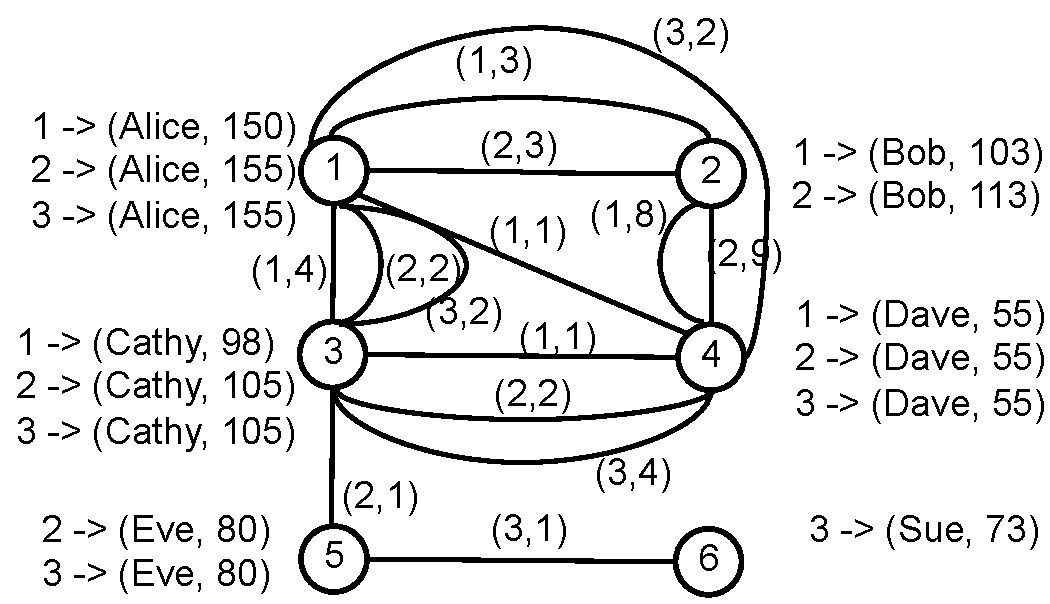
\includegraphics[width=2.2in]{figs/mg.pdf}
\caption{MG for T1.}
\label{fig:mg}
\end{minipage}
\begin{minipage}{2.3in}
\centering
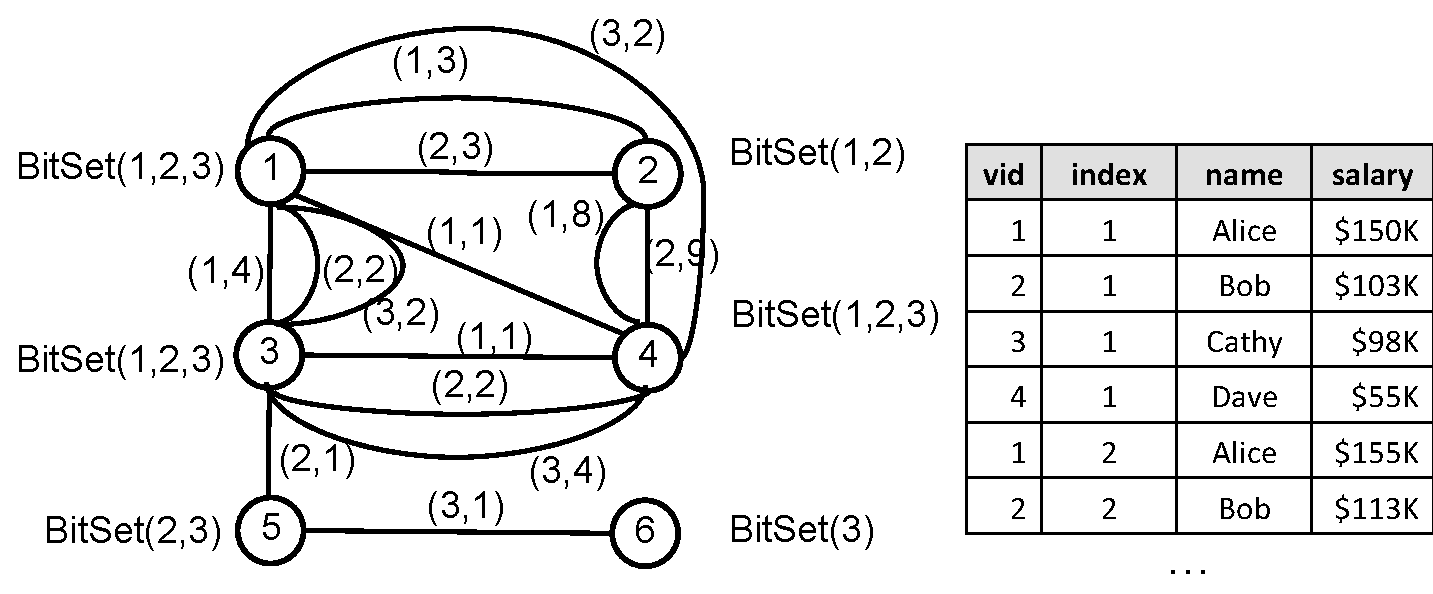
\includegraphics[width=2.2in]{figs/mgc.pdf}
\caption{MGC for T1.}
\label{fig:mgc}
\end{minipage}
\begin{minipage}{2.3in}
\centering
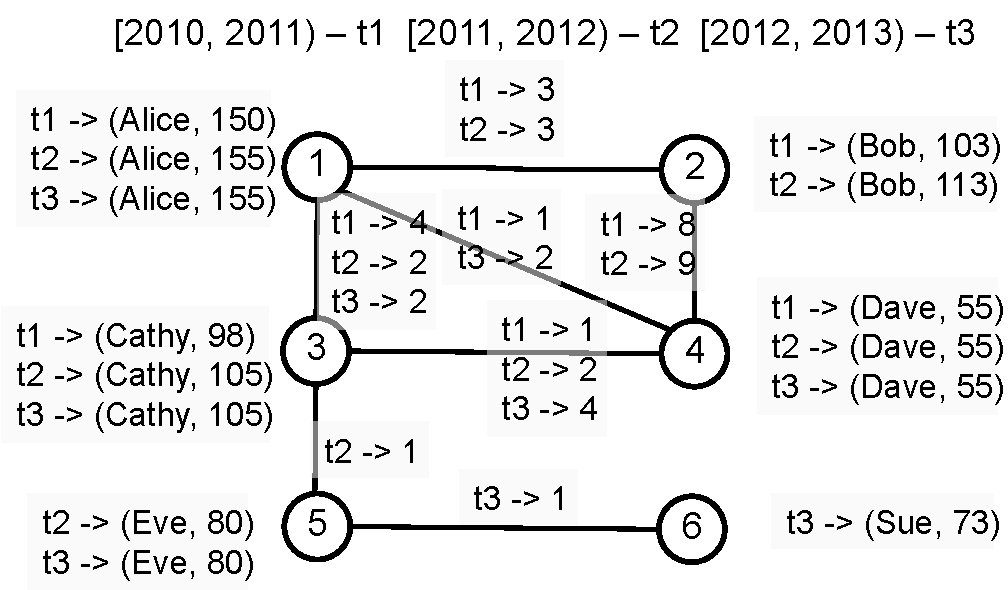
\includegraphics[width=2.2in]{figs/og.pdf}
\caption{OG for T1.}
\label{fig:og}
\end{minipage}
\end{figure*}

\subsection{Query Optimization}
\label{sec:sys:optimization}

The operations are generally applied in the following order: tselect,
tgroup, tunion, and finally, analytics and projection.  In some cases,
an equivalent result can be achieved by processing tunion prior to
tgroup.  For example, an intersection of two evolving graphs with a
small temporal overlap, followed by a tgroup, will usually lead to a
more efficient execution.  \vera{if we have time, we could show this
  experimentally.}  The difficulty is that this change of order can lead
to incorrect result, and thus should be applied in such as a way as to
assure correctness (or not applied at all).

In addition to selecting the most efficient order of operations, we
select the best data structure for the query.  Our analysis of data
structures' effectiveness for each individual operation is shown in
the next section.  Switching between data structures from operation to
operation is possible but computationally inefficient.  Instead, we
pick the structure that provides the best compromise for the query
operations by associating costs with each operation and picking the
least expensive one.  \vera{I made that up but it sounds possible.}

In our experience, the partitioning of the data affects the
performance more than the data structure choice itself.  A poor
partition strategy, in terms of the correct number of partitions and
the allocation of edges to partitions, can be 10x times slower than a
good one, as we show in the next section.  We evaluated different
strategies and partition numbers experimentally and this serves as a
basis of a second dimension of the cost model.

Other criteria that can affect the query performance are data skew,
change rate between snapshots, and data size.  We continue to evaluate
these aspects and will incorporate them into the query optimization.


\subsection{Data Representation}
\label{sec:sys:datastructs}

We developed several in-memory representations of evolving graphs to
explore the trade-offs of compactness, parallelism, and support of
different query operators. \eat{ The data structures represent a
  continuum of replication, from the SnapshotGraph to OneGraph and are
  described here in more detail.}

{\bf SnapshotGraph (SG).} The simplest way to represent an evolving
graph is by representing each snapshot individually, a direct
translation of our logical data model.  We call this data structure
SnapshotGraph, or SG for short. An example of an SG is depicted in
Figure~\ref{fig:sgp}.  SG is a collection of snapshots, where vertices
and edges store the attribute values for the specific time interval.
A \insql{TSelect} operation on this representation is a slice of the
snapshot sequence, while \insql{TGroup} and temporal joins
(\insql{TAnd} and \insql{TOr}) require a group by key within each
aggregate set of vertices and edges.

While the SG representation is simple, it is not compact, considering
that in many real-world evolving graphs there is a 80\% or larger
similarity between consecutive
snapshots~\cite{DBLP:journals/tos/MiaoHLWYZPCC15}.  In a distributed
architecture, however, this data structure provides some benefits as
operations on it can be easily parallelized, by assigning different
snapshots to different workers, or by partitioning a snapshot across
workers.  \eat{with improved temporal locality for snapshot-based
  analytics. }\eat{SG edges can be partitioned using temporal or
  structural criteria.  Furthermore, due to Spark's lazy evaluation,
  operations such as \insql{TSelect} are very efficient, since only
  those snapshots involved in the operation are loaded.  While other
  data structures do not benefit from this feature, push selection in
  query optimization can compensate equally well.}

{\bf MultiGraph (MG).}  To take advantage of high similarity between
snapshots, we developed another data structure called MultiGraph, or
MG for short (Figure~\ref{fig:mg}).  MG stores the evolving graph as a
single graph, with one vertex for all time periods, but with one edge
per period where it exists.  Because our goal is to represent both
topological and attribute information, we need to store not only
vertex presence or absence (which can be easily accomplished by an
existence string, like in~\cite{Kan2009}, or by bit sets), but also
the values of vertex attributes at each time period.  MG vertex
attribute, thus, is a map of time indices that represent intervals to
corresponding values.  Edge attributes are tuples of the time index
and the corresponding value.  Vertices typically change infrequently,
so storing each vertex only once reduces the total number of vertices
by about 80\% in our data.  Some of these savings, however, are taken
up by the storage of a more complex map data structure for attribute
values, compared to a single attribute as in SG.  \eat{Partition of
  the MG edges can be either temporal or structural, which lead to
  different rates of vertex replication between partitions.}

The implementation of some of the \ql operations in MG is more complex
than in SG.  \insql{TSelect} is a subgraph operation that operates on
all vertices and edges.  \insql{TGroup} on vertices is a combination
of transform and filter operations, since the vertices are already
aggregated across the whole time period, but the edges, like in SG,
are grouped by key within their respective sets.  Implementation of
snapshot analytics like PageRank is done in batch mode, similar
to~\cite{DBLP:journals/tos/MiaoHLWYZPCC15}, by computing the values
and sending messages between vertices for all time periods at once.
\eat{This data structure should also be more amenable to cross-time
analytics and pattern mining, which we intend to explore in the
future.}

Note that for a large subset of the queries, attribute information is
not used, and only the topology is important.  Thus, we can store
vertex attributes in a separate collection (column store), removing
the attribute map and replacing it with existence bit sets instead.
This is the essence of the special case of MultiGraph, called {\bf
  MultiGraphColumn (MGC)}, depicted in Figure~\ref{fig:mgc}.  The MGC
representation allows storage of an arbitrary number of vertex
attributes without using complex per-vertex lists, read from disk only
as needed, and so amenable to lazy evaluation, an important
performance optimization in Apache Spark.  Further compression can be
achieved by storing vertex attribute values only once across all time
periods in which they are the same, similar to how temporal databases
represent this type of data (e.g., see~\cite{Muller2008}).  The
drawback of this approach is that decompression is required to
support, for example, the \insql{TGroup} operation.

\eat{\begin{figure}[t!]
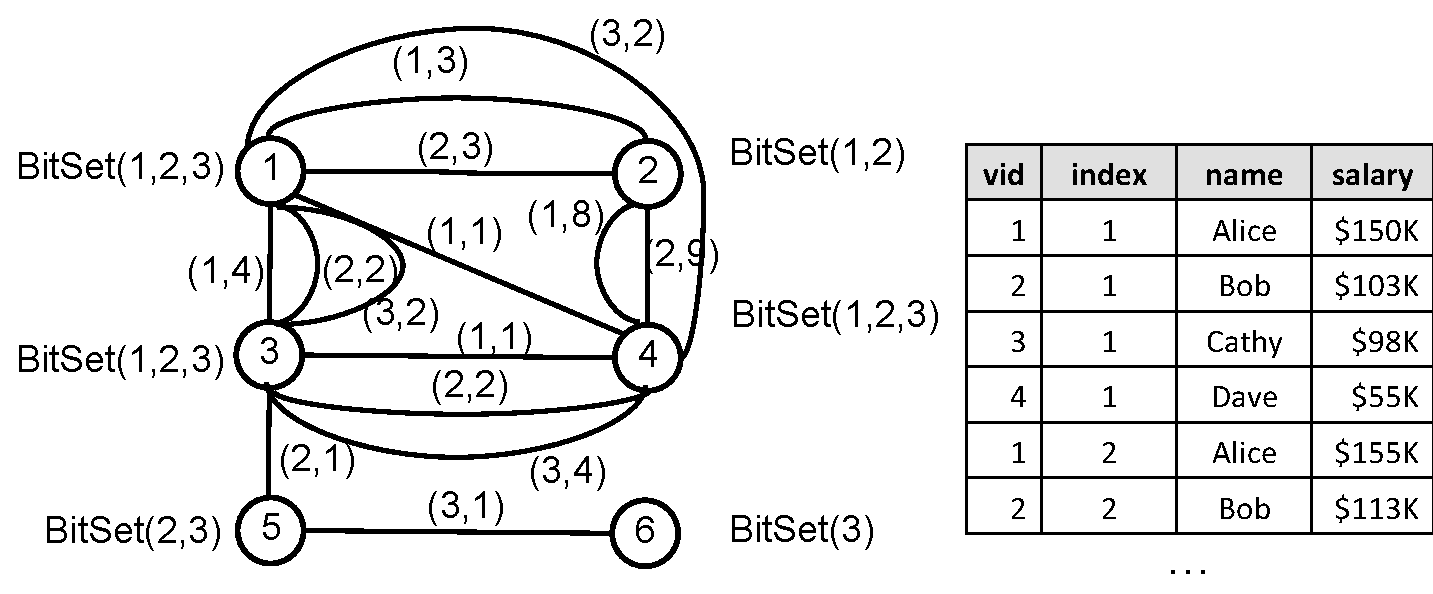
\includegraphics[width=3.2in]{figs/mgc.pdf}
\caption{MGC representation of T1 from Figure~\ref{fig:tg}.}
\label{fig:mgc}
\end{figure}}

{\bf OneGraph (OG).}  The most topologically compact representation is
to store each vertex {\em and} each edge only once for the whole
evolving graph, by taking a union of the snapshot vertex and edge
sets.  The OneGraph data structure, or OG for short, uses this
representation in our system.  Similar to MG, vertex and edge
attributes are stored in time-indexed maps (Figure~\ref{fig:og}).
Compared to MG, this leads to storing about 75\% fewer edges.  The OG
data structure provides some benefits in addition to compactness,
since it reduces the total communication between vertices in
Pregel-based analytics in batch mode.  The drawback is that OG is much
denser than individual snapshots.  As with MG, \insql{TSelect} is a
subgraph operation, and \insql{TGroup} is a transform and filter
operation --- for both vertices and edges.

\eat{\begin{figure}[t!]
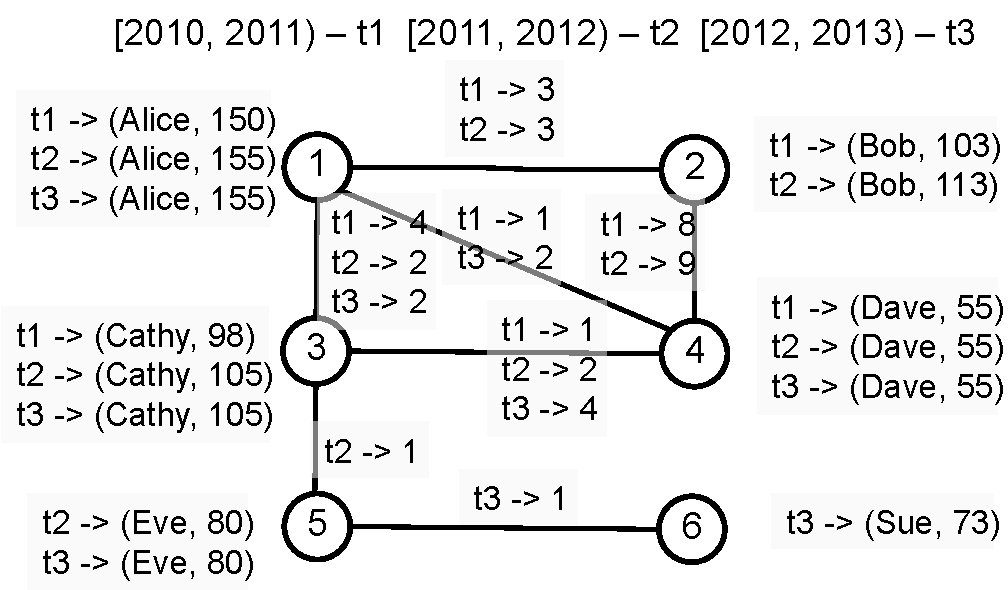
\includegraphics[width=3.2in]{figs/og.pdf}
\caption{OG of T1 from~\ref{fig:tg}.}
\label{fig:og}
\end{figure}}

Similar to MGC, {\bf OneGraphColumn (OGC)} uses a single graph to
represent the union of vertices and edges, with bit sets for presence
information, while attribute information is stored separately.  This
is not as compact as storing attributes within the graph elements, but
is faster in many operations where only graph topology is required.

\begin{figure*}
\begin{minipage}{2.3in}
\centering
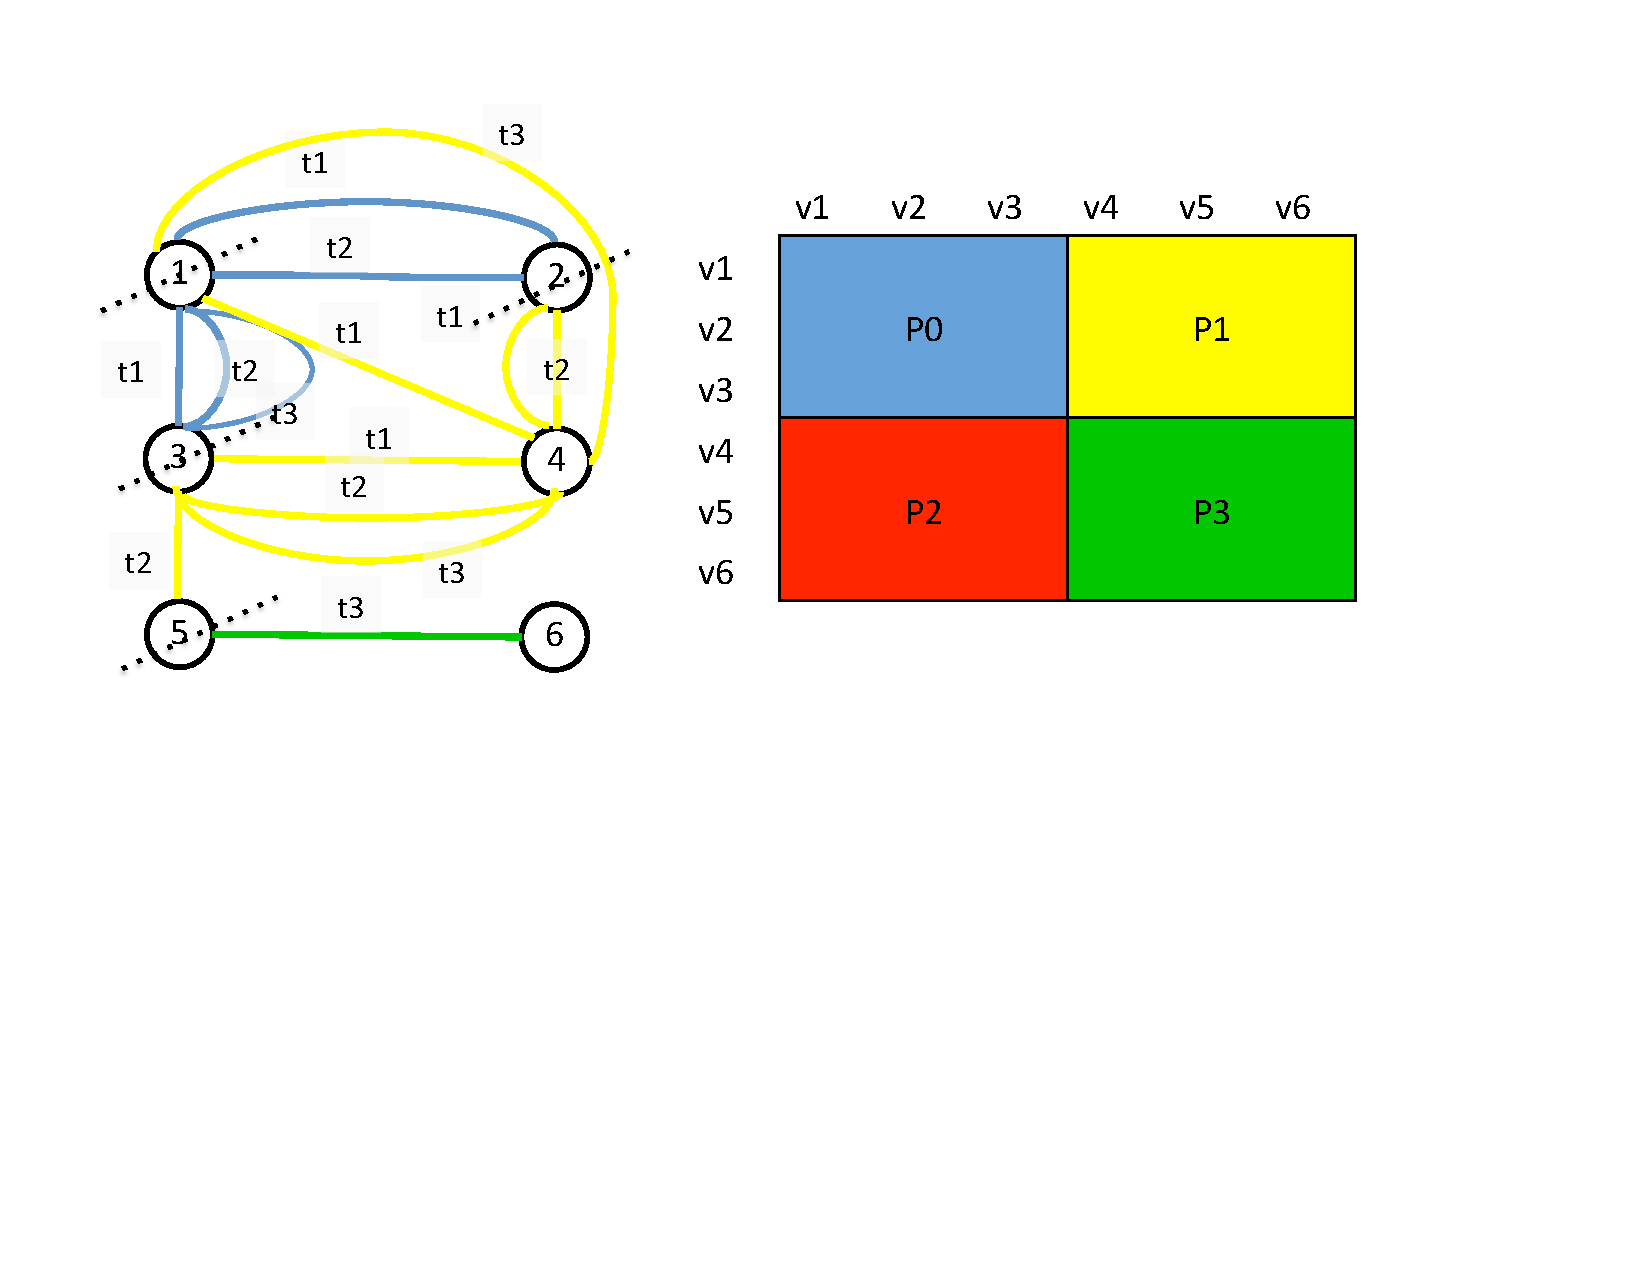
\includegraphics[width=2.3in]{figs/E2D_1.pdf}
\caption{E2D with 4 partitions.}
\label{fig:e2d}
\end{minipage}
\begin{minipage}{2.3in}
\centering
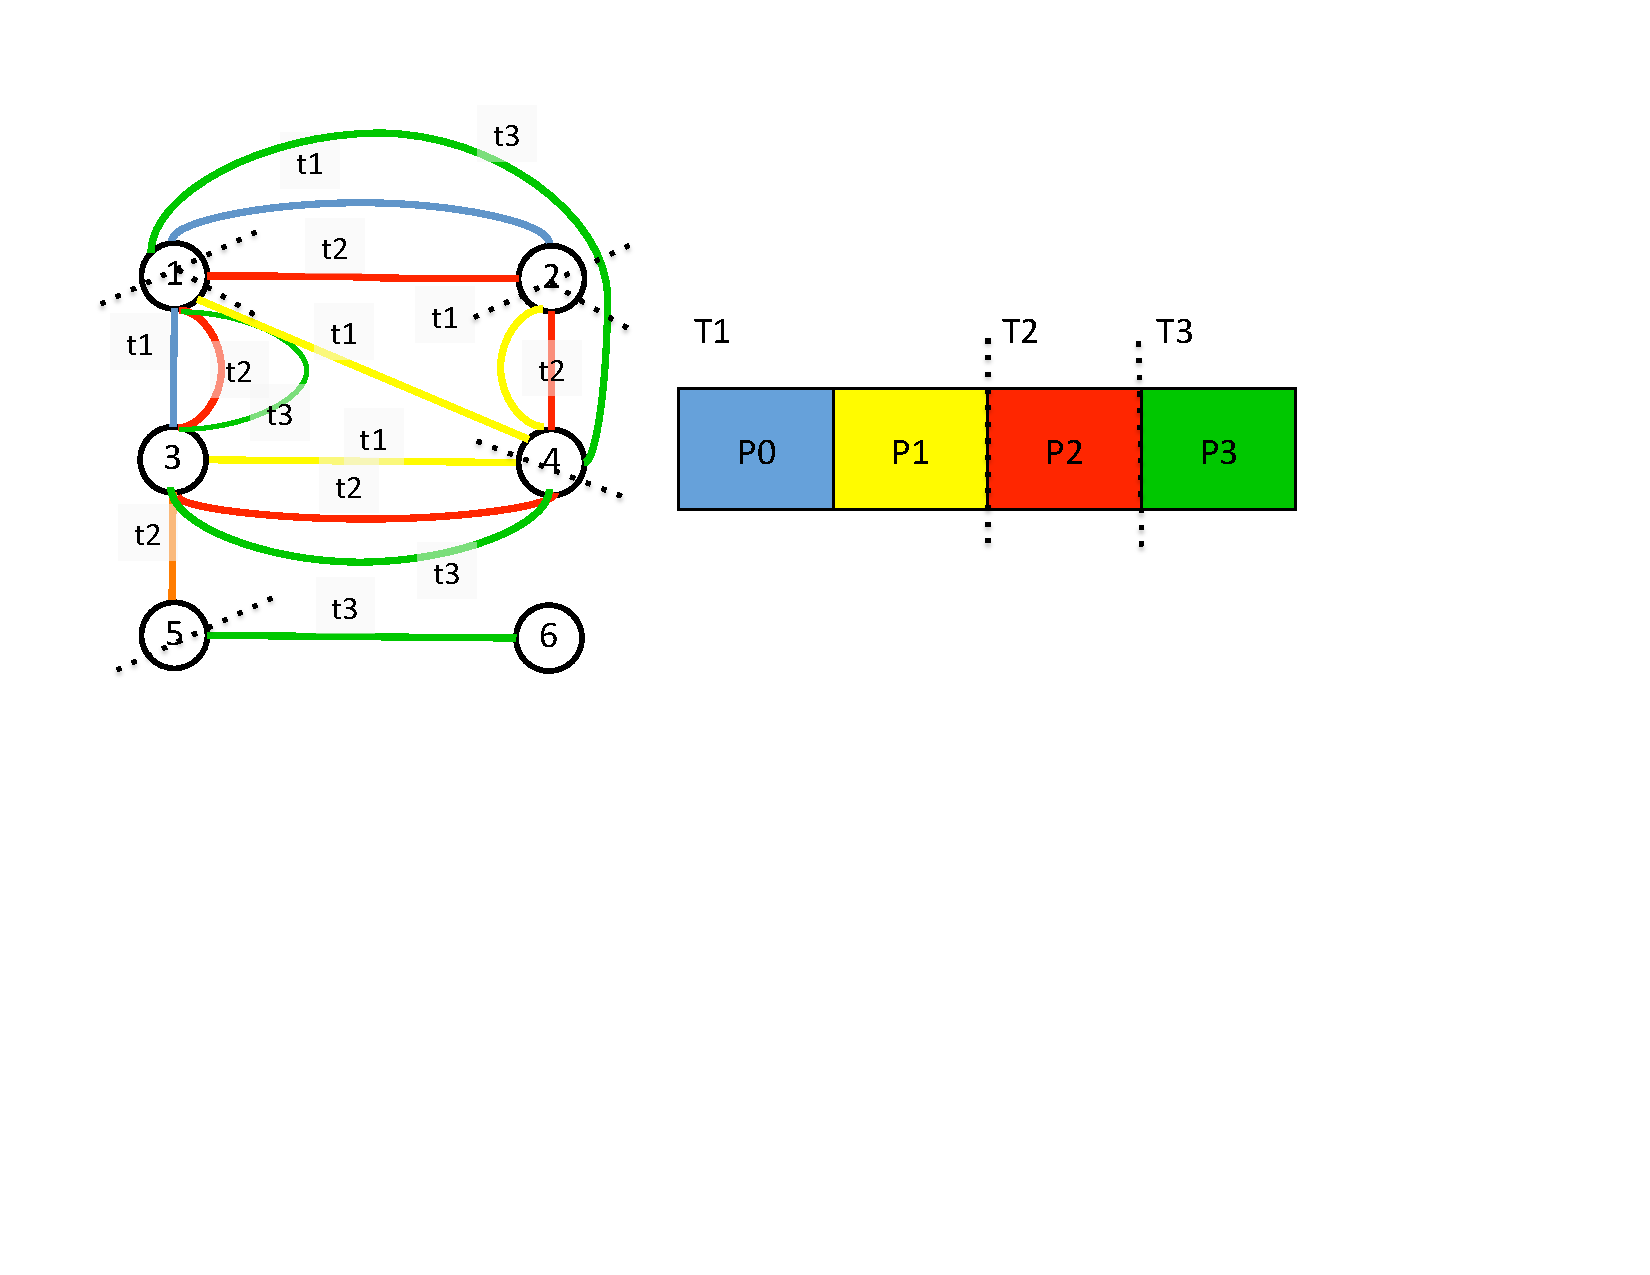
\includegraphics[width=2.3in]{figs/Consecutive_1.pdf}
\caption{Consecutive with 4 partitions, 3 snapshots.}
\label{fig:consecutive}
\end{minipage}
\begin{minipage}{2.2in}
\centering
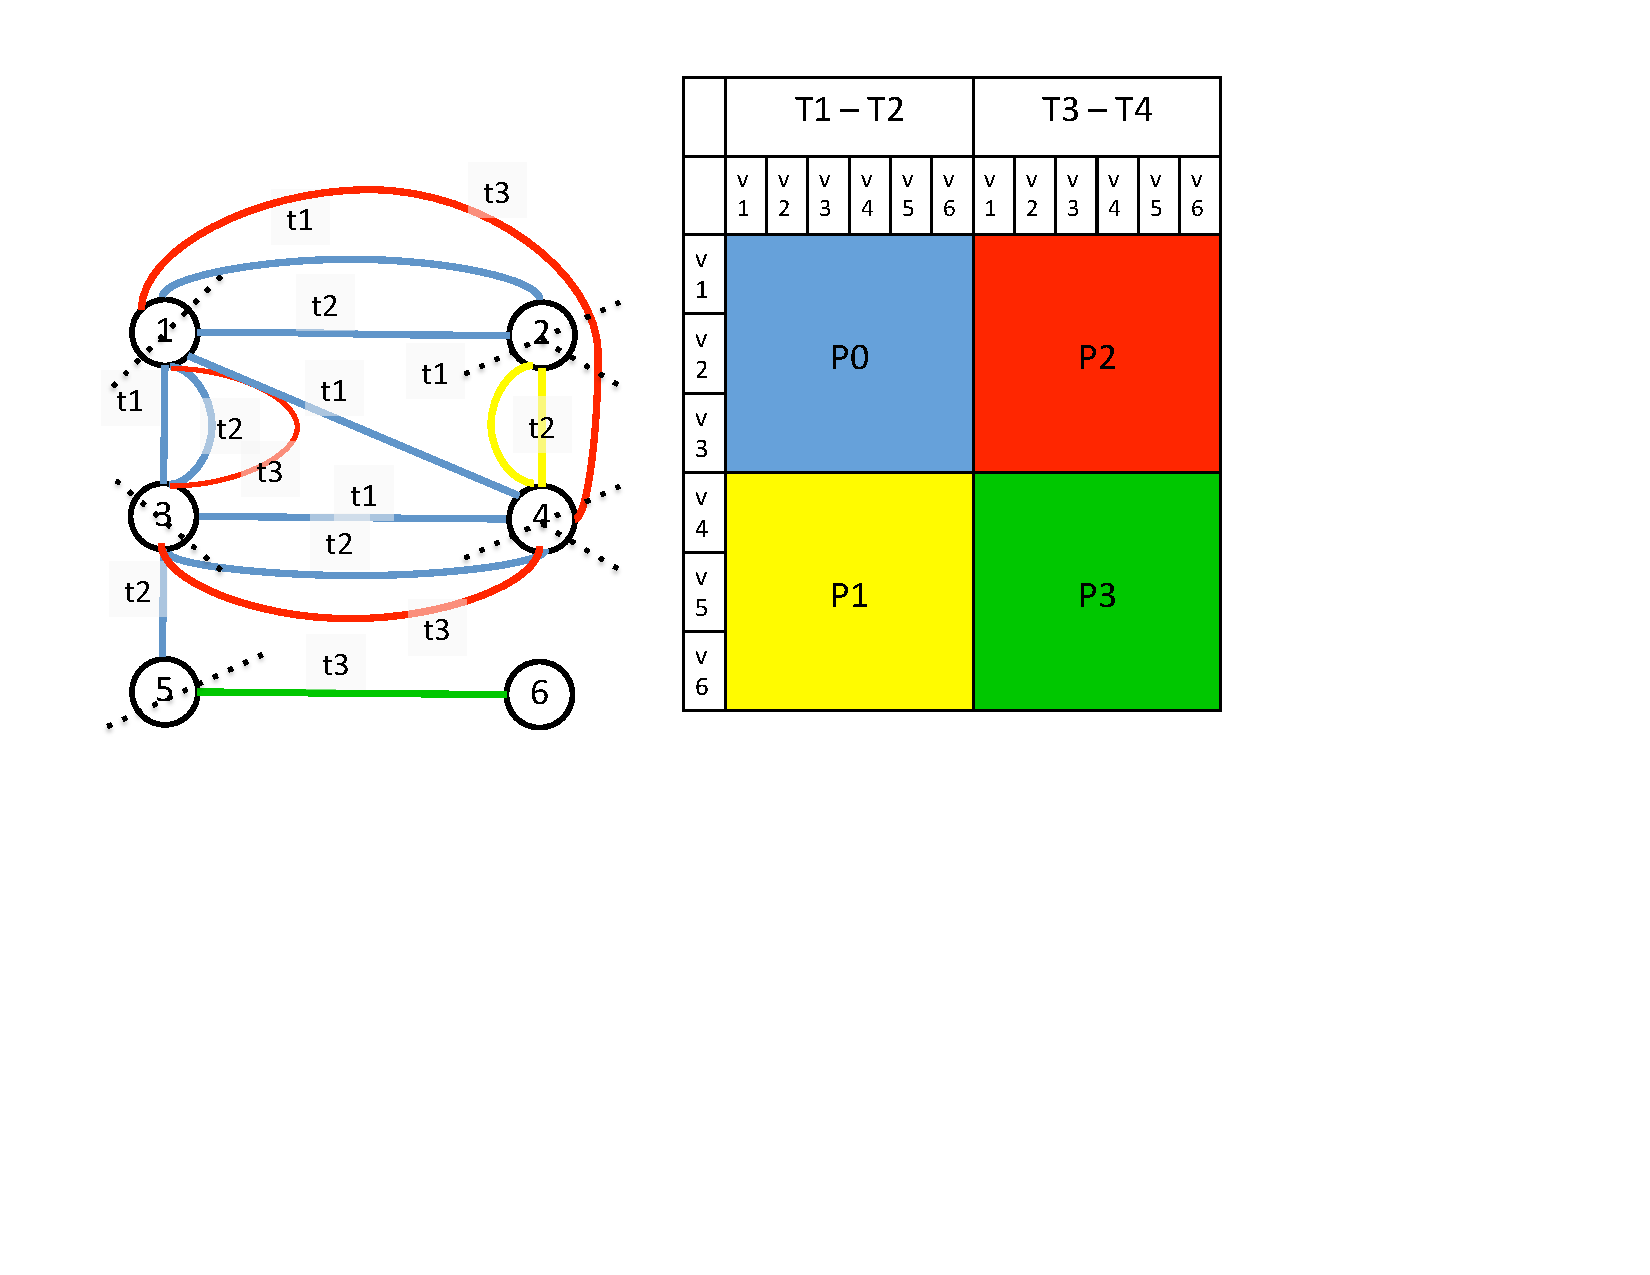
\includegraphics[width=2.2in]{figs/Hybrid2D_1.pdf}
\caption{E2D-Temporal with 4 partitions, 4 snapshots, 2 runs.}
\label{fig:hybrid2d}
\end{minipage}
\end{figure*}

\subsection{Partitioning Strategies}  
\label{sec:sys:partition}

Graph partitioning can have a tremendous impact on system performance.
A good partitioning strategy needs to (1) be balanced, assigning an
approximately equal number of units to each partition, and (2) limit
the number of cuts across partitions, to reduce cross-partition
communication.  

There are two basic types of graph partitioning strategies. Vertex-cut
(also known as edge partitioning) distributes edges across the
available machines and replicates vertices as necessary, while
edge-cut (vertex partitioning) does the opposite.  Vertex-cut
approaches have been shown to have better
performance~\cite{Gonzalez2012}, and are the strategies of choice in
Graph X.  In \ql, we support six different vertex-cut strategies,
which are applied prior to the operation but after loading, and can be
re-applied at any point.

{\bf Canonical Random Vertex Cut (CRVC).}  The source and destination
ids of a vertex are hashed in a canonical direction and the result is
distributed among the available partitions.  The result is a random
vertex cut that co-locates all edges connecting a given pair of
vertices, regardless of direction.  This strategy is available in
GraphX and was used without modification.

{\bf 2D Edge (E2D).}  A sparse edge adjacency matrix is partitioned in
two dimensions (Figure~\ref{fig:e2d}), guaranteeing a $2 \sqrt{n}$
bound on vertex replication, where $n$ is the number of
partitions. E2D can provide good performance for Pregel-style
analytics.  This strategy is available in GraphX and was used without
modification.

\eat{\begin{figure}[t!]
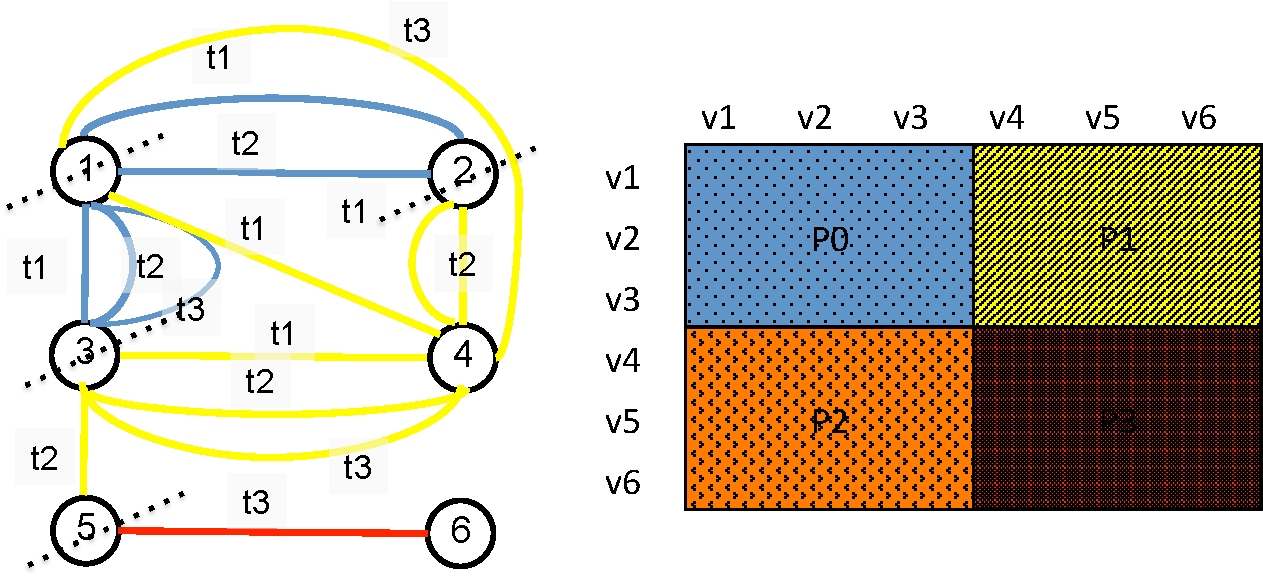
\includegraphics[width=3.2in]{figs/E2D.pdf}
\caption{E2D partitioning over 4 partitions.}
\label{fig:e2d}
\end{figure}}

{\bf Naive Temporal.} Let $n$ be the number of snapshots and $p$ be
the number of partitions.  If $n \geq p$, then snapshot $i$ is placed
into partition $i \% p$.  Otherwise, multiple partitions are grouped
into a {\em run}, and the CRVC strategy is used to partition a
snapshot within each run.

\eat{ Provided there are more time intervals in the graph than there
  are partitions, each edge is placed in the time index modulo number
  of partitions place, round-robin fashion.  In the case where the
  graph covers a small time interval, multiple partitions are used for
  each interval (we term this a {\em run}), and the CRVC strategy is
  applied within each run.}

{\bf Consecutive Temporal.}  Let $n$ be the number of snapshots and
$p$ be the number of partitions.  If $n \geq p$, then temporally
consecutive snapshots are assigned to the same partition.  Otherwise,
each snapshot is assigned an equal number of consecutive partitions,
and CRVC is used to partition the snapshot
(Figure~\ref{fig:consecutive}).

\eat{If there are more time intervals than partitions, consecutive
  time intervals are assigned to the same partition in runs.  If there
  are more partitions, each time interval is assigned an equal number
  of consecutive partitions, within which CRVC strategy is applied
  (Figure~\ref{fig:consecutive}).} 

Many networks exhibit strong temporal skew, with later snapshots being
significantly larger than earlier ones.  Consecutive temporal strategy
may result in an unbalanced partitioning for networks with large skew.

Furthermore, the number of cuts for a vertex is the number of
intervals in which it exists with degree > 0.  In the worst case, a
vertex will be cut $n$ times.  Therefore, if vertices persist across
many time intervals, this strategy is not a good choice.

\eat{\begin{figure}[t!]
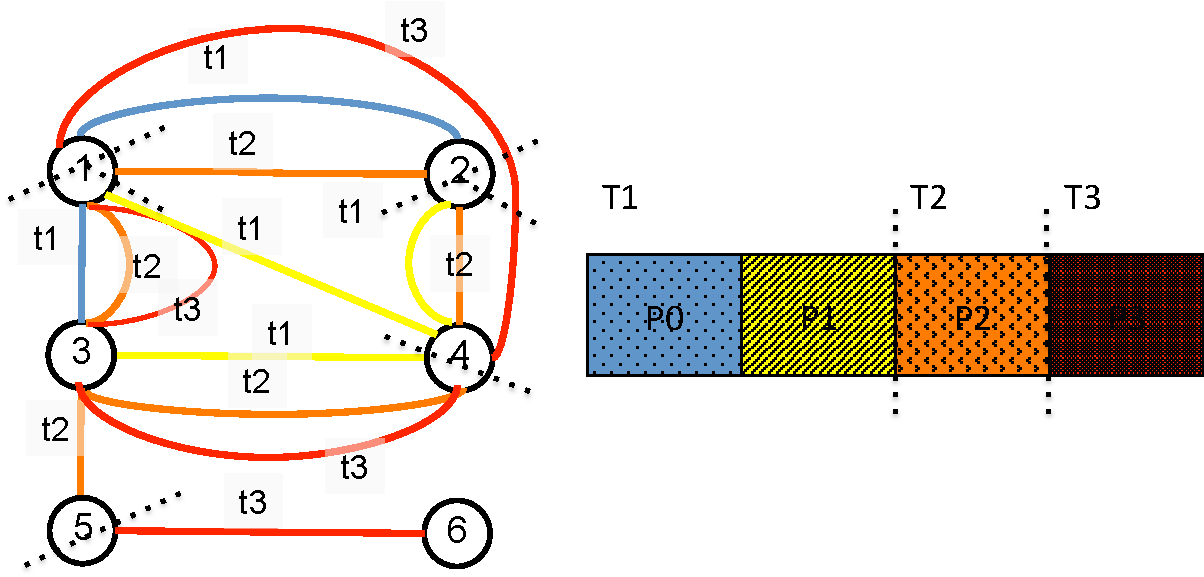
\includegraphics[width=3.2in]{figs/Consecutive.pdf}
\caption{Consecutive strategy over 4 partitions and 3 time intervals.}
\label{fig:consecutive}
\end{figure}}

{\bf Hybrid strategies.} Hybrid strategies combine elements of
temporal and structural criteria.  We define two such strategies,
E2D-Temporal (Figure~\ref{fig:hybrid2d}) and CRVC-Temporal.  With both
strategies, we create runs of temporally consecutive snapshots, assign
an equal number of partitions to each run, and then use E2D or CRVC
within each run.

These strategies are specifically designed for time-based operations
such as aggregation to co-locate edges that are to be grouped.  Run
width is determined based on the operation.  For \insql{TGroup}, we
take the number of snapshots in a group as the run width.  For other
operations the default run width is 2.

\eat{
\begin{figure}[t!]
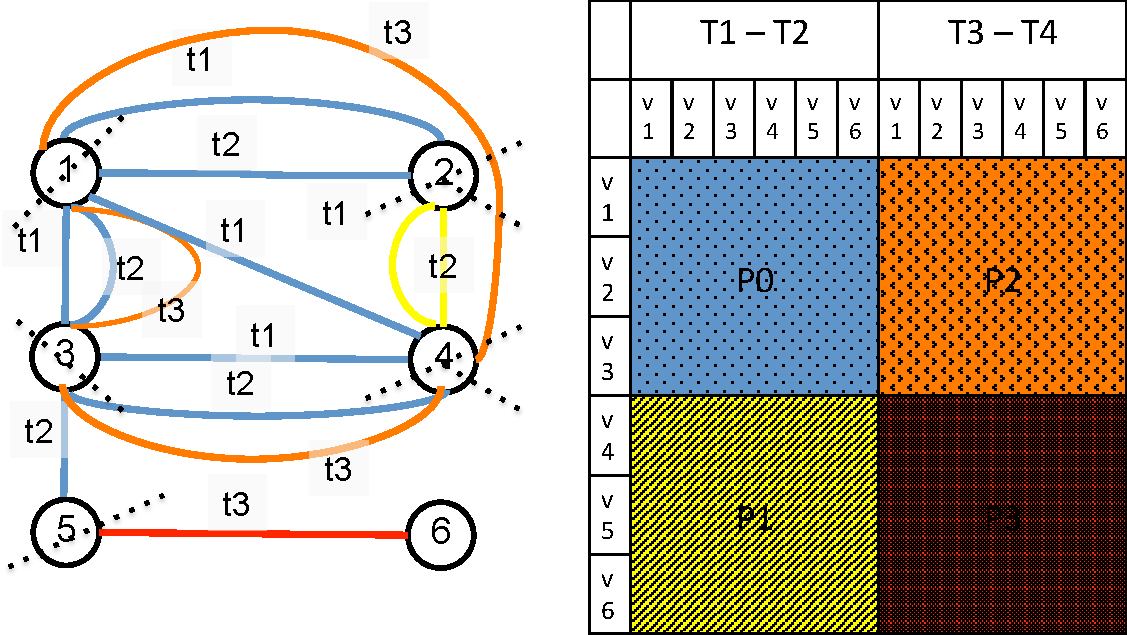
\includegraphics[width=3.2in]{figs/Hybrid2D.pdf}
\caption{Hybrid 2D Edge Temporal strategy over 4 partitions and 4 time
  intervals in runs of width 2.}
\label{fig:hybrid2d}
\end{figure}}

Note that not all partitioning strategies can be applied to every data
structure.  For example, only purely structural strategies can be
applied to OG.  We report on the experimental effectiveness of the
strategies in Section~\ref{sec:exp}.


